%Este trabalho está licenciado sob a Licença Atribuição-CompartilhaIgual 4.0 Internacional Creative Commons. Para visualizar uma cópia desta licença, visite http://creativecommons.org/licenses/by-sa/4.0/deed.pt_BR ou mande uma carta para Creative Commons, PO Box 1866, Mountain View, CA 94042, USA.

\chapter{Aplicações da derivada}\label{cap_apderiv}
\thispagestyle{fancy}

\ifispython
\begin{obs}\label{obs:cap_apderiv_python}
  Nos códigos \sympy~ apresentados neste capítulo, assumimos o seguinte preâmbulo:
\begin{verbatim}
from sympy import *
var('x',real=True)
\end{verbatim}
\end{obs}
\fi

\section{Regra de L'Hôpital}\label{cap_apderiv_sec_lhospital}

A regra de L'Hôpital é uma técnica para o cálculo de limites de indeterminações. Sejam $f$ e $g$ funções deriváveis em um intervalo aberto contendo $x=a$, exceto possivelmente em $x=a$, e
\begin{equation}
  \lim_{x\to a} f(x) = 0\quad\text{e}\quad\lim_{x\to a} g(x) = 0.
\end{equation}
Se, ainda, $\lim_{x\to a} f(x)/g(x)$ existe ou for $\pm\infty$, então
\begin{equation}
  \lim_{x\to a} \frac{f(x)}{g(x)} = \lim_{x\to a} \frac{f'(x)}{g'(x)}.
\end{equation}
Esta é a versão da regra de L'Hôpital para indeterminações do tipo $0/0$. Sem grandes modificações, é diretamente estendida para os casos $x\to a^-$, $x\to a^+$, $x\to \infty$ e $x\to -\infty$.

\begin{ex}
  Vamos calcular o limite
  \begin{equation}
    \lim_{x\to 1} \frac{x-1}{x^2-1}.
  \end{equation}
  \begin{enumerate}[a)]
  \item Pela regra de L'Hôpital.
    \begin{align}
      \lim_{x\to 1} \frac{x-1}{x^2-1} &= \lim_{x\to 1} \frac{(x+1)'}{(x^2-1)'} \\
                                      &= \lim_{x\to 1} \frac{1}{2x} \\
                                      &= \frac{1}{2}.
    \end{align}
  \item Por eliminação do fator comum.
    \begin{align}
      \lim_{x\to 1} \frac{x-1}{x^2-1} &= \lim_{x\to 1} \frac{x-1}{(x-1)(x+1)} \\
                                      &= \lim_{x\to 1} \frac{1}{x+1} \\
                                      &= \frac{1}{2}.
    \end{align}
  \end{enumerate}

  \ifispython
  No \sympy\footnote{Veja a Observação \ref{obs:cap_apderiv_python}.}, temos
\begin{verbatim}
>>> limit((x-1)/(x**2-1),x,1)
1/2
\end{verbatim}
  \fi
\end{ex}

\begin{ex}
  O limite
  \begin{equation}
    \lim_{x\to 2} \frac{x^2-4x+4}{x^3-3x^2+4}
  \end{equation}
  é uma indeterminação $0/0$. Aplicando a regra de L'Hôpital, obtemos
  \begin{equation}
    \lim_{x\to 2} \frac{x^2-4x+4}{x^3-3x^2+4} = \lim_{x\to 2} \frac{\cancelto{0}{2x-4}}{\cancelto{0}{3x^2-6x}},
  \end{equation}
  que também é uma indeterminação do tipo $0/0$. Agora, aplicando a regra de L'Hôpital novamente, obtemos
  \begin{equation}
    \lim_{x\to 2} \frac{2x-4}{3x^2-6x} = \lim_{x\to 2} \frac{2}{6x-6} = \frac{1}{3}.
  \end{equation}
  Portanto, concluímos que
  \begin{equation}
    \lim_{x\to 2} \frac{x^2-4x+4}{x^3-3x^2+4} = \frac{1}{3}.
  \end{equation}  

  \ifispython
  No \sympy\footnote{Veja a Observação \ref{obs:cap_apderiv_python}.}, temos
\begin{verbatim}
>>> limit((x**2-4*x+4)/(x**3-3*x**2+3),x,2)
1/3
\end{verbatim}
  \fi
\end{ex}

\begin{obs}
  A regra de L'Hôpital também pode ser usada para indeterminações do tipo $\infty/\infty$.
\end{obs}

\begin{ex}
  Vamos calcular
  \begin{equation}
    \lim_{x\to \infty} \frac{e^x}{x},
  \end{equation}
  que é uma indeterminação do tipo $\infty/\infty$. Então, aplicando a regra de L'Hôpital, temos
  \begin{equation}
    \lim_{x\to \infty} \frac{e^x}{x} = \lim_{x\to \infty} \frac{e^x}{1} = \infty.
  \end{equation}
\end{ex}

\subsection*{Exercícios resolvidos}

\begin{exeresol}
  Calcule
  \begin{equation}
    \lim_{x\to 0^-} \frac{e^x-1}{x^2}.
  \end{equation}
\end{exeresol}
\begin{resol}
  Observamos tratar-se de uma indeterminação do tipo $0/0$, i.e.
  \begin{equation}
    \lim_{x\to 0^-} \frac{\cancelto{0}{e^x-1}}{\cancelto{0}{x^2}}.
  \end{equation}
  Então, aplicando a regra de L'Hôpital, temos
  \begin{equation}
    \lim_{x\to 0^-} \frac{e^x-1}{x^2} = \lim_{x\to 0^-} \frac{\cancelto{1}{e^x}}{\cancelto{0^-}{2x}} = -\infty.
  \end{equation}
\end{resol}

\begin{exeresol}(Indeterminação do tipo $0\cdot\infty$)

  Calcule
  \begin{equation}
    \lim_{x\to \infty} x^{51}e^{-x}.
  \end{equation}
\end{exeresol}
\begin{resol}
  Observamos que
  \begin{equation}
    \lim_{x\to \infty} \cancelto{\infty}{x^{51}}\cancelto{0}{e^{-x}} = \lim_{x\to \infty} \frac{\cancelto{\infty}{x^{51}}}{\cancelto{\infty}{e^{x}}}.
  \end{equation}
  Então, aplicando a regra de L'Hôpital sucessivamente, obtemos
  \begin{align}
    \lim_{x\to\infty} x^{51}e^{-x} &= \lim_{x\to\infty} \frac{x^{51}}{e^x} \\
                                   &= \lim_{x\to\infty} \frac{51\cdot x^{50}}{e^x} \\
                                   &= \lim_{x\to\infty} \frac{51\cdot 50\cdot x^{49}}{e^x} \\
                                   &\vdots \\
                                   &= \lim_{x\to\infty} \frac{51!}{\cancelto{\infty}{e^x}} = 0.
  \end{align}
\end{resol}

\begin{exeresol}(Indeterminação do tipo $\infty - \infty$)

  Calcule
  \begin{equation}
    \lim_{x\to 0^+} \left(\frac{1}{x} - \frac{1}{e^x-1}\right).
  \end{equation}
\end{exeresol}
\begin{resol}
  Trata-se de uma indeterminação do tipo $\infty - \infty$, pois
  \begin{equation}
    \lim_{x\to 0^+} \left(\cancelto{\infty}{\frac{1}{x}} - \cancelto{\infty}{\frac{1}{e^x-1}}\right).
  \end{equation}
  Neste caso, calculando a subtração, obtemos
  \begin{align}
    \lim_{x\to 0^+} \left(\frac{1}{x} - \frac{1}{e^x-1}\right) &= \lim_{x\to 0^+} \frac{e^x-1+x}{xe^x-x},
  \end{align}
  a qual é uma indeterminação do tipo $0/0$. Aplicando a regra de L'Hôpital, obtemos
  \begin{align}
    \lim_{x\to 0^+} \frac{e^x-1-x}{xe^x-x} &= \lim_{x\to 0^+} \frac{\cancelto{0}{e^x-1}}{\cancelto{0}{(x+1)e^x-1}} \\
                                           &= \lim_{x\to 0^+} \frac{e^x}{(x+2)e^x} \\
    &= \lim_{x\to 0^+} \frac{1}{x+2} = \frac{1}{2}.
  \end{align}
\end{resol}

\begin{exeresol}(Indeterminação do tipo $1^\infty$)

  Calcule
  \begin{equation}
    \lim_{x\to 0^+} (1+x)^{1/x}.
  \end{equation}
\end{exeresol}
\begin{resol}
  Trata-se de uma indeterminação do tipo $1^\infty$. Em tais casos, a seguinte estratégia pode ser útil. Nos pontos de continuidade da função logaritmo natural, temos
  \begin{align}
    \ln\left(\lim_{x\to 0^+} (1+x)^{1/x}\right) &= \lim_{x\to 0^+} \ln\left((1+x)^{1/x}\right) \\
                                                &= \lim_{x\to 0^+} \frac{\cancelto{0}{\ln(1+x)}}{\cancelto{0}{x}} \\
                                                &= \lim_{x\to 0^+} \frac{\frac{1}{x+1}}{1} = 1.
  \end{align}
  Ou seja,
  \begin{equation}
    \ln\left(\lim_{x\to 0^+} (1+x)^{1/x}\right) = 1 \Rightarrow \lim_{x\to 0^+} (1+x)^{1/x} = e.
  \end{equation}
\end{resol}

\subsection*{Exercícios}

\begin{exer}
  Calcule
  \begin{equation}
    \lim_{x\to -1} \frac{x+1}{x^2+3x+2}.
  \end{equation}
\end{exer}
\begin{resp}
  $1$
\end{resp}

\begin{exer}
  Calcule
  \begin{equation}
    \lim_{x\to \infty} x^{-51}e^x.
  \end{equation}
\end{exer}
\begin{resp}
  $\infty$
\end{resp}

\begin{exer}
  Calcule
  \begin{equation}
    \lim_{x\to 0^+} \left(\frac{1}{x}+\ln x\right).
  \end{equation}
\end{exer}
\begin{resp}
  $\infty$
\end{resp}

\begin{exer}
  Calcule
  \begin{equation}
    \lim_{x\to 0^+} \left(e^x + x\right)^{\frac{1}{2x}}.
  \end{equation}
\end{exer}
\begin{resp}
  $e$
\end{resp}

\section{Extremos de funções}\label{cap_apderiv_sec_extfun}

Seja $f$ uma função com domínio $D$. Dizemos que $f$ tem o valor \emph{máximo global}\footnote{Também chamado de máximo absoluto.} $f(a)$ no ponto $x=a$ quando
\begin{equation}
  f(x) < f(a),
\end{equation}
para todo $x\in D\setminus\{a\}$. Analogamente, dizemos que $f$ tem o valor \emph{mínimo global}\footnote{Também chamado de mínimo absoluto.} $f(b)$ no ponto $x=b$ quando
\begin{equation}
  f(x) > f(b),
\end{equation}
para todo $x\in D\setminus\{b\}$. Em tais pontos, dizemos que a função têm seus valores \emph{extremos globais} (ou extremos absolutos).

\begin{ex}\label{ex:vmaxminabs}
  A função $f(x) = x^2$ tem valor mínimo global no ponto $x=0$ e não assume valor máximo global. A função $g(x) = -x^2$ tem valor máximo global no ponto $x=0$ e não assume valor mínimo global. A função $h(x)=x^3$ não assume valores mínimo e máximo globais. Veja a Figura \ref{fig:ex_vmaxminabs}.

  \begin{figure}[H]
    \centering
    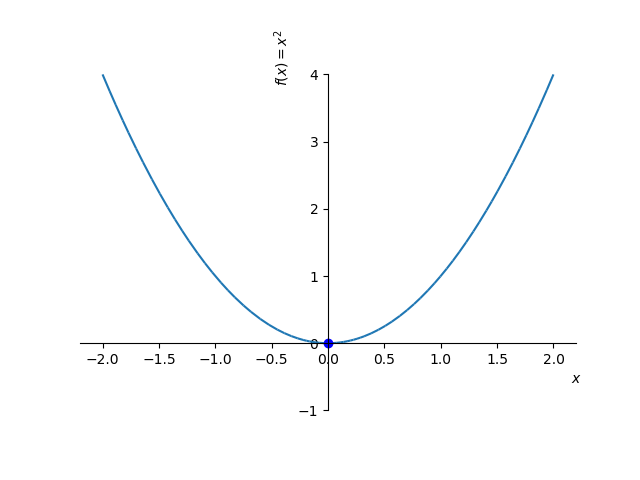
\includegraphics[width=0.32\textwidth]{./cap_apderiv/dados/fig_ex_vmaxminabs/fig_f}~
    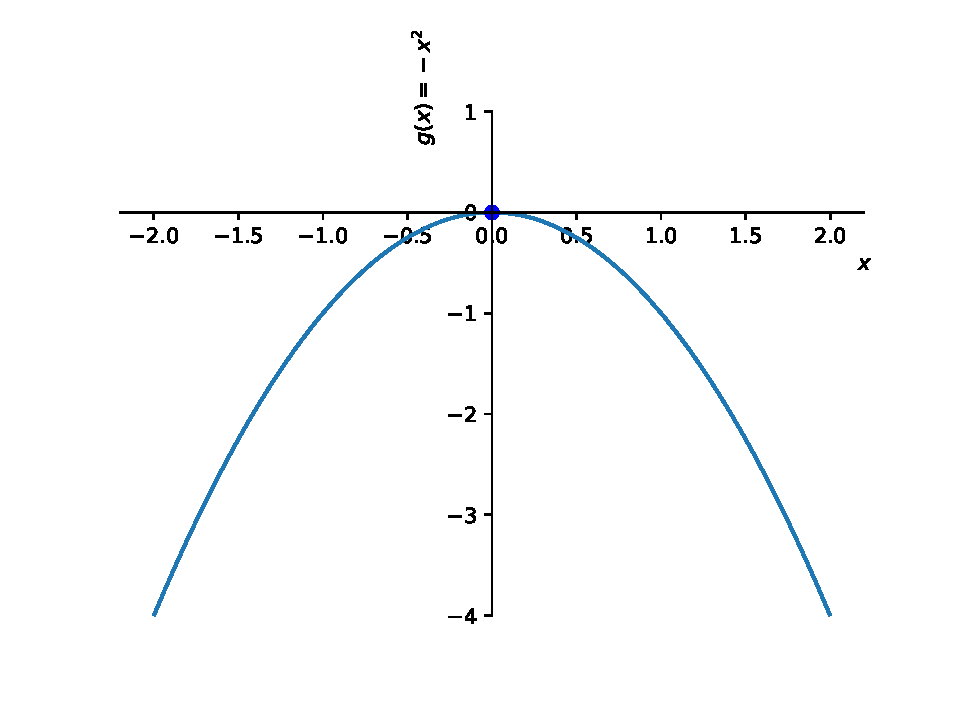
\includegraphics[width=0.32\textwidth]{./cap_apderiv/dados/fig_ex_vmaxminabs/fig_g}~
    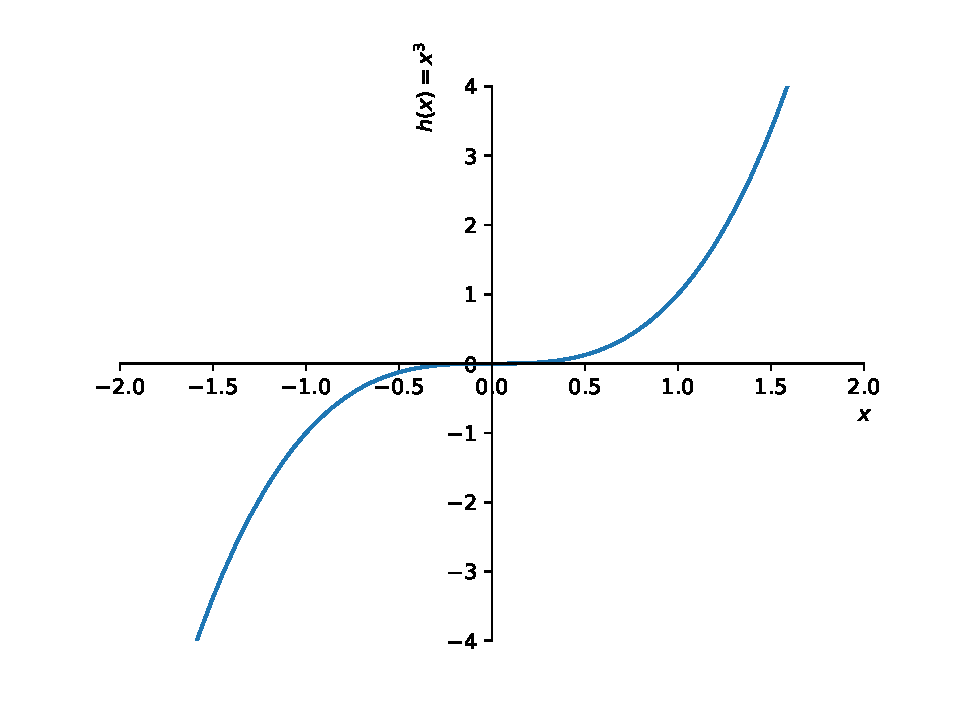
\includegraphics[width=0.32\textwidth]{./cap_apderiv/dados/fig_ex_vmaxminabs/fig_h}
    \caption{Esboço das funções discutidas no Exemplo \ref{ex:vmaxminabs}.}
    \label{fig:ex_vmaxminabs}
  \end{figure}
\end{ex}

\begin{teo}\normalfont{(Teorema do valor extremo)}
  Se $f$ é uma função contínua em um intervalo fechado $[a, b]$, então $f$ assume tanto um valor máximo como um valor mínimo global em $[a, b]$.
\end{teo}

\begin{ex}\label{ex:fcont}
  Vejamos os seguintes casos:
  \begin{enumerate}[a)]
  \item  A função $\pmb{f(x) = (x-1)^2+1}$ é contínua no intervalo fechado $\displaystyle \left[0, \frac{3}{2}\right]$. Assume valor mínimo global $1$ no ponto $x=1$. Ainda, assume valor máximo global igual a $2$ no ponto $x=0$. Veja Figura \ref{fig:ex_fcont_f}.
  \begin{figure}[H]
    \centering
    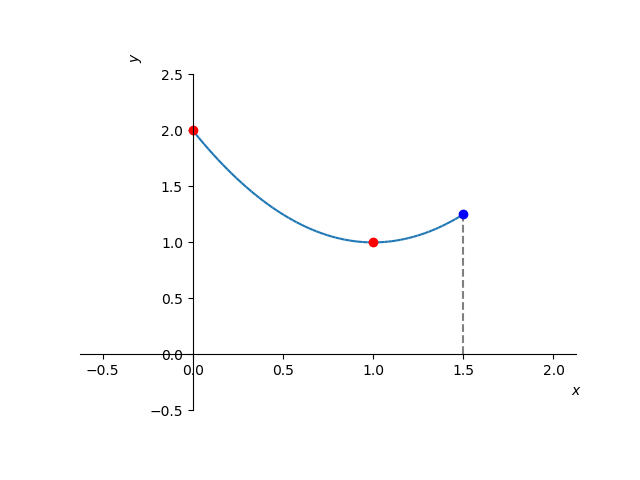
\includegraphics[width=0.7\textwidth]{./cap_apderiv/dados/fig_ex_fcont/fig_f}
    \caption{Esboço do gráfico de $f(x) = (x-1)^2+1$ no intervalo $\displaystyle\left[0, \frac{3}{2}\right]$. Veja o Exemplo \ref{ex:fcont} a).}
    \label{fig:ex_fcont_f}
  \end{figure}
\item A função $\pmb{g(x) = \ln x}$ é contínua no intervalo $(0, e]$. Neste intervalo, assume valor máximo global no ponto $x=e$, mas não assume valor mínimo global. Veja Figura \ref{fig:ex_fcont_g}.
  \begin{figure}[H]
    \centering
    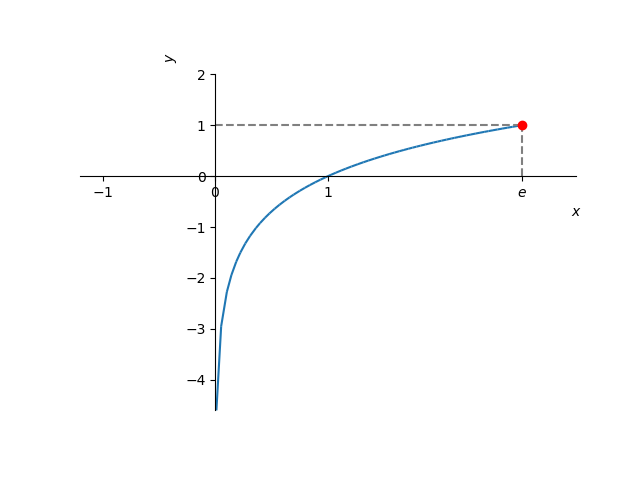
\includegraphics[width=0.7\textwidth]{./cap_apderiv/dados/fig_ex_fcont/fig_g}
    \caption{Esboço do gráfico de $g(x) = \ln x$ no intervalo $(0,e]$. Veja o Exemplo \ref{ex:fcont} b).}
    \label{fig:ex_fcont_g}
  \end{figure}
  
\item A função
  \begin{equation}
    h(x) = \left\{
      \begin{array}{ll}
        x &, 0\leq x < 1,\\
        0 &, x=1,
      \end{array}
\right.
\end{equation}
definida no intervalo $[0, 1]$ é descontínua no ponto $x=1$. Neste intervalo, assume valor mínimo global no ponto $x=0$, mas não assume valor máximo global. Veja a Figura \ref{fig:ex_fcont_h}.
  \begin{figure}[H]
    \centering
    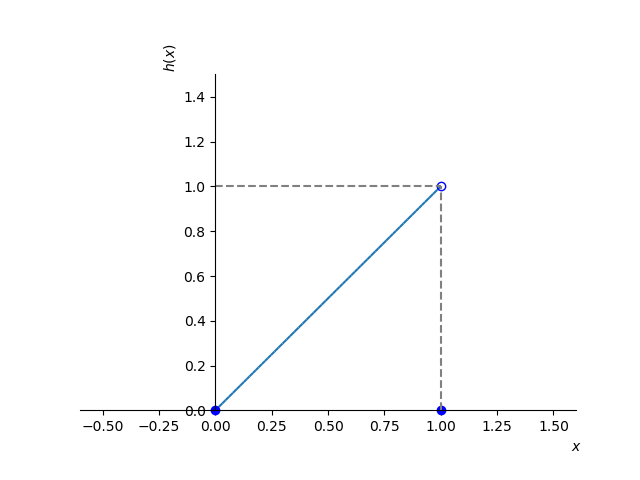
\includegraphics[width=0.7\textwidth]{./cap_apderiv/dados/fig_ex_fcont/fig_h}
    \caption{Esboço do gráfico de $h(x)$ no intervalo $[0,1]$. Veja o Exemplo \ref{ex:fcont} c).}
    \label{fig:ex_fcont_h}
  \end{figure}
  \end{enumerate}
\end{ex}

Uma função $f$ tem um valor \emph{máximo local} em um ponto interior $x=a$ de seu domínio, se $f(x) < f(a)$ para todo $x$ em um intervalo aberto em torno de $a$, excluindo-se $x=a$. Analogamente, $f$ tem um valor \emph{mínimo local} em um ponto interior $x=b$ de seu domínio, se $f(x) > f(b)$  para todo $x$ em um intervalo aberto em torno de $b$, excluindo-se $x=b$. Em tais pontos, dizemos que a função têm valores \emph{extremos locais} (ou relativos). Um tal ponto é chamado de \emph{ponto de máximo local} ou \emph{de mínimo local}, conforme o caso.

\begin{ex}\label{ex:vmaxminloc}
  Consideremos a função
  \begin{equation}
    f(x) = \left\{
      \begin{array}{ll}
        -(x+1)^2-2 &, -2\leq x < -\frac{1}{2},\\
        |x| &, -\frac{1}{2} \leq x < 1,\\
        (x-2)^3+2 &, 1\leq x < 3.
      \end{array}
\right.
\end{equation}

  \begin{figure}[H]
    \centering
    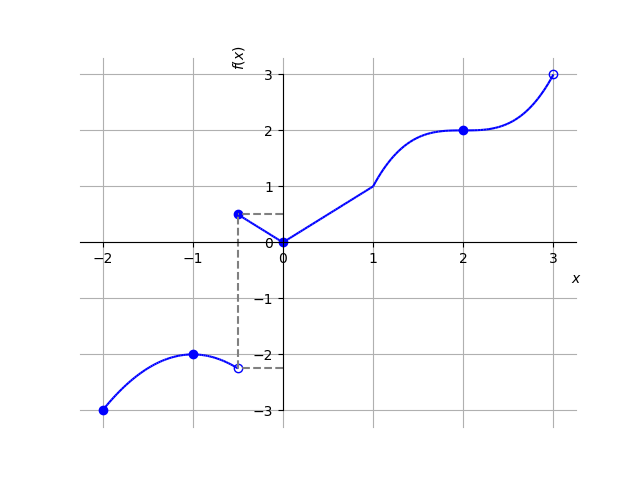
\includegraphics[width=0.7\textwidth]{./cap_apderiv/dados/fig_ex_vmaxminloc/fig_f}
    \caption{Esboço do gráfico de $f(x)$ discutida no Exemplo \ref{ex:vmaxminloc}.}
    \label{fig:ex_vmaxminloc}
  \end{figure}
  
Na Figura \ref{fig:ex_vmaxminloc} temos o esboço de seu gráfico. Por inferência, temos que $f$ tem valores máximos locais nos pontos $x=-1$ e $x=-1/2$. No ponto $x=0$ tem um valor mínimo local. Observamos que $x=-2$, $x=2$ e $x=3$ não são pontos de extremos locais desta função. No ponto $x=-2$, $f$ tem seu valor mínimo global. Ainda, $f$ não tem valor máximo global.
\end{ex}

\begin{teo}\normalfont{(Teorema da derivada para pontos extremos locais.)}
  Se $f$ possui um valor extremo local em um ponto $x=a$ e $f$ é diferenciável neste ponto, então
  \begin{equation}
    f'(a) = 0.
  \end{equation}
\end{teo}

Deste teorema, podemos concluir que uma função $f$ pode ter valores extremos em:
\begin{enumerate}
\item pontos interiores de seu domínio onde $f' = 0$,
\item pontos interiores de seu domínio onde $f'$ não existe, ou
\item pontos extremos de seu domínio.
\end{enumerate}

Um ponto interior do domínio de uma função $f$ onde $f'=0$ ou $f'$ não existe, é chamado de \emph{ponto crítico} da função.

\begin{obs}\label{obs:pt_critico_val_extremo}
  Uma função tem valores extremos em pontos críticos ou nos extremos de seu domínio.
\end{obs}


\begin{ex}
  Consideramos a função $f(x)$ discutida no Exemplo \ref{ex:vmaxminloc}. No ponto $x=-1$, $f'(-1)=0$ e $f$ tem valor máximo local neste ponto. Entretanto, no ponto $x=2$, também temos $f'(2)=0$, mas $f$ não tem valor extremo neste ponto.

  No ponto $x=0$, $f'(0)$ não existe e $f$ tem valor mínimo local neste ponto. No ponto, $x=-1/2$, $f'(1/2)$ não existe e $f$ tem valor máximo local neste ponto.

  Nos extremos do domínio, temos que $f$ tem valor mínimo global no ponto $x=-2$, mas não tem extremo global no ponto $x=3$.
\end{ex}

\subsection*{Exercícios resolvidos}

\begin{exeresol}\label{exeresol:f_diff}
  Determine os pontos extremos da função $f(x) = (x+1)^2-1$ no intervalo $[-2,1]$.
\end{exeresol}
\begin{resol}
  Os valores extremos de um função podem ocorrer, somente, em seus pontos críticos ou nos extremos de seu domínio. Como $f(x) = (x+1)^2-1$ é diferenciável no intervalo $(-2,1)$, seus pontos críticos são pontos tais que $f'=0$. Para identificá-los, calculamos
  \begin{align}
    f'(x)=0 &\Rightarrow 2(x+1) = 0\\
            &\Rightarrow x = -1.
  \end{align}

  \begin{figure}[H]
    \centering
    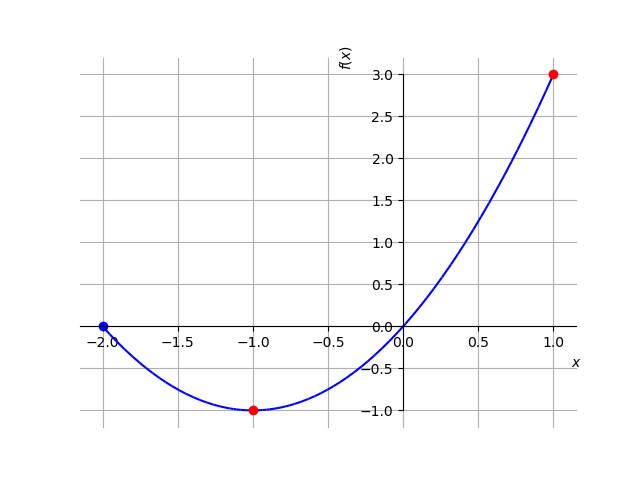
\includegraphics[width=0.7\textwidth]{./cap_apderiv/dados/fig_exeresol_f_diff/fig_exeresol_f_diff}
    \caption{Esboço do gráfico da função $f(x) = (x+1)^2-1$ discutida no Exercício Resolvido \ref{exeresol:f_diff}.}
    \label{fig:exeresol_f_diff}
  \end{figure}

  Desta forma, $f$ pode ter valores extremos nos ponto $x=-2$, $x=-1$ e $x=1$. Analisamos, então, o esboço do gráfico da função (Figura \ref{fig:exeresol_f_diff}) e a seguinte tabela:\\
  \begin{center}
  \begin{tabular}[H]{l|ccc}
    $x$ & -2 & -1 & 1 \\\hline
    $f(x)$ & 0 & -1 & 3\\\hline
  \end{tabular}
\end{center}
Daí, podemos concluir que $f$ tem o valor mínimo global (e local) de $f(-1)=-1$ no ponto $x=-1$ e tem valor máximo global de $f(1)=3$ no ponto $x=1$.

\ifispython
Podemos usar o \sympy~para computar os pontos extremos e plotar a função. Por exemplo, com os seguintes comandos\footnote{Veja a Observação \ref{obs:cap_apderiv_python}.}:
\begin{verbatim}
>>> f = (x+1)**2-1, f
>>> f = (x+1)**2-1; f
(x + 1)**2 - 1
>>> fl = diff(f,x); fl
2*x + 2
>>> xc = solve(fl,x); xc
[-1]
>>> f.subs(x,-2); f.subs(x,-1); f.subs(x,1)
>>> plot(f,(x,-2,1))
\end{verbatim}
\fi
\end{resol}

\begin{exeresol}\label{exeresol:p_infl}
  Determine os pontos extremos da função $f(x)=x^3$ no intervalo $[-1, 1]$.
\end{exeresol}
\begin{resol}
  Como $f$ é diferenciável no intervalo $(-1, 1)$, temos que seus pontos críticos são tais que $f'(x)=0$. Neste caso, temos
  \begin{equation}
    3x^2=0\Rightarrow x=0
  \end{equation}
  é o único ponto crítico de $f$. Entretanto, analisando o gráfico desta função (Figura \ref{fig:exeresol_p_infl}) vemos que $f$ não tem valor extremo local neste ponto. Assim, seus pontos extremos só podem ocorrer nos extremos do domínio $[-1, 1]$. Concluímos que $f(-1)=-1$ é o valor mínimo global de $f$ e $f(1)=1$ é seu valor máximo global.

  \begin{figure}[H]
    \centering
    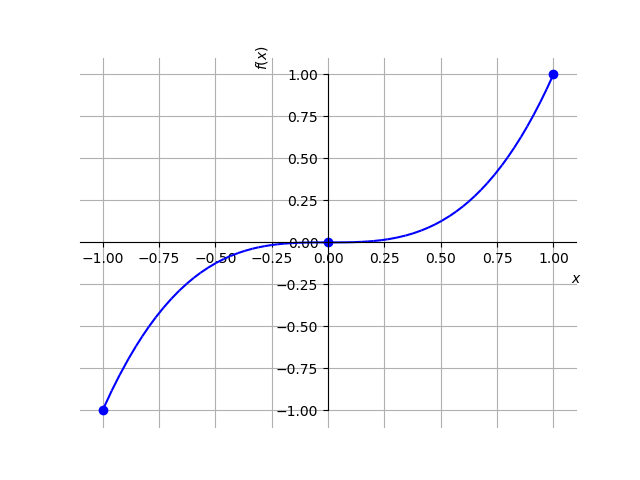
\includegraphics[width=0.7\textwidth]{./cap_apderiv/dados/fig_exeresol_p_infl/fig_exeresol_p_infl}
    \caption{Esboço do gráfico da função $f(x) = x^3$ discutida no Exercício Resolvido \ref{exeresol:p_infl}.}
    \label{fig:exeresol_p_infl}
  \end{figure}
\end{resol}

\subsection*{Exercícios}

\begin{exer}
  Considere que uma dada função $f$ tenha o seguinte esboço de gráfico:

  \begin{center}
    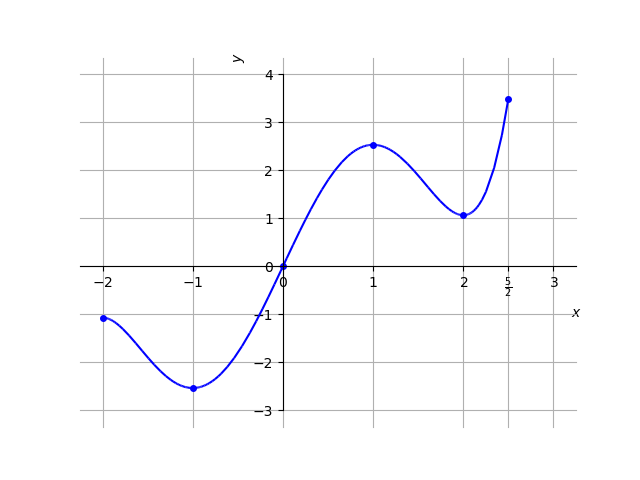
\includegraphics[width=0.7\textwidth]{./cap_apderiv/dados/fig_exer_extfun/fig_exer_extfun}
  \end{center}

  Determine e classifique os pontos extremos desta função.
\end{exer}
\begin{resp}
  $x=-1$ ponto de mínimo global; $x=1$ ponto de máximo local; $x=2$ ponto de mínimo local; $x=\frac{5}{2}$ ponto de máximo global.
\end{resp}

\begin{exer}
  Dada a função $f(x)=x^2-2x+3$ restrita ao intervalo $[-1,2]$, determine:
  \begin{enumerate}[a)]
  \item seu(s) ponto(s) crítico(s).
  \item seu(s) ponto(s) extremo(s) e o(s) classifique.
  \item seu(s) valor(es) extremo(s) e o(s) classifique.
  \end{enumerate}
\end{exer}
\begin{resp}
  a)~$x=1$; b)~$x=-1$ ponto de máximo global; $x=1$ ponto de mínimo local e global; c)~$f(-1)=6$ valor máximo global; $f(1)=2$ valor mínimo local e global;
\end{resp}

\begin{exer}
  Dada a função $f(x)=-x^2+2x+1$ restrita ao intervalo $[0,3]$, determine:
  \begin{enumerate}[a)]
  \item seu(s) ponto(s) crítico(s).
  \item seu(s) ponto(s) extremo(s) e o(s) classifique.
  \item seu(s) valor(es) extremo(s) e o(s) classifique.
  \end{enumerate}
\end{exer}
\begin{resp}
  a)~$x=1$; b)~$x=1$ ponto de máximo local e global; $x=3$ ponto de mínimo global; c)~$f(1)=2$ valor máximo local e global; $f(3)=-2$ valor mínimo global;
\end{resp}

\begin{exer}
  Dada a função $f(x)=x^{3} - 3 x^{2} + 3 x$ restrita ao intervalo $[0, \infty)$, determine:
  \begin{enumerate}[a)]
  \item seu(s) ponto(s) crítico(s).
  \item seu(s) ponto(s) extremo(s) e o(s) classifique.
  \item seu(s) valor(es) extremo(s) e o(s) classifique.
  \end{enumerate}
\end{exer}
\begin{resp}
  a)~$x=1$; b)~$x=0$ ponto de mínimo global;c)~$f(0)=0$ valor mínimo global;
\end{resp}

\begin{exer}
  Dada a função $f(x)=x^{1/3}$ restrita ao intervalo $[-1,1]$, determine:
  \begin{enumerate}[a)]
  \item seu(s) ponto(s) crítico(s).
  \item seu(s) ponto(s) extremo(s) e o(s) classifique.
  \item seu(s) valor(es) extremo(s) e o(s) classifique.
  \end{enumerate}
\end{exer}
\begin{resp}
  a)~$x=0$; b)~$x=-1$ ponto de mínimo global; $x=1$ ponto de máximo global; c)~$f(-1)=-1$ valor mínimo global; $f(1)=1$ valor máximo global;
\end{resp}


\section{Teorema do valor médio}\label{cap_apderiv_sec_valormedio}

O teorema do valor médio é uma aplicação do teorema de Rolle.

\subsection{Teorema de Rolle}

O teorema de Rolle fornece uma condição suficiente para que uma dada função diferenciável tenha derivada nula em pelo menos um ponto.

\begin{figure}[H]
  \centering
  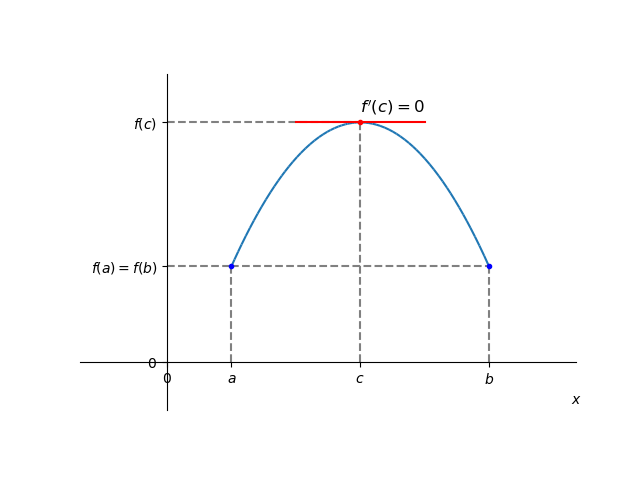
\includegraphics[width=0.7\textwidth]{./cap_apderiv/dados/fig_teo_Rolle/fig_teo_Rolle}
  \caption{Ilustração do teorema de Rolle.}
  \label{fig:teo_Rolle}
\end{figure}

\begin{teo}\normalfont{(Teorema de Rolle)}
  Seja $f$ uma função contínua no intervalo fechado $[a, b]$ e diferenciável no intervalo aberto $(a, b)$. Se
  \begin{equation}
    f(a)=f(b),
  \end{equation}
  então existe pelo menos um ponto $c\in (a, b)$ tal que
  \begin{equation}
    f'(c)=0.
  \end{equation}
\end{teo}

\begin{ex}
  Vejamos os seguintes casos:
  \begin{enumerate}[a)]
  \item O polinômio $p(x) = x^3 - 4x^2 + 3x$ tem pelo menos um ponto crítico no intervalo $(0,1)$ e no intervalo $(1,3)$. De fato,
    \begin{align}
      p(x) &= x^3 - 4x^2 + 3x\\
           &= x(x^2 - 4x + 3)\\
           &= x(x-1)(x-3).
    \end{align}
    Logo, temos $p(0)=p(1)=0$ e, pelo teorema de Rolle, segue que existe pelo menos um ponto $c\in (0, 1)$ tal que $f'(c)=0$. Analogamente, como $p(1)=p(3)=0$, segue do teorema que existe pelo menos um ponto crítico no intervalo $(1,3)$.
  \end{enumerate}
\item A função
  \begin{equation}
    f(x) = \left\{
      \begin{array}{ll}
        x &, 0\leq x < 1,\\
        0 &, x=1.
      \end{array}
\right.
\end{equation}
é tal que $f(0)=f(1)=0$, entretanto sua derivada $f'(x)=1$ no intervalo $(0, 1)$. Ou seja, a condição da $f$ ser contínua no intervalo fechado associado é necessária no teorema de Rolle.
\item Não existe ponto tal que a derivada da $g(x)=-|x-1|+1$ seja nulo. Entretanto, notemos que $g(0)=g(2)=0$ e $g$ contínua no intervalo fechado $[0, 2]$. O teorema de Rolle não se aplica neste caso, pois $g$ não é diferenciável no intervalo $(0,2)$, mais especificamente, no ponto $x=1$.
\end{ex}

\subsection{Teorema do valor médio}

O teorema do valor médio é uma generalização do teorema de Rolle.

\begin{teo}\normalfont{(Teorema do valor médio)}
  Seja $f$ uma função contínua no intervalo fechado $[a,b]$ e diferenciável no intervalo aberto $(a,b)$. Então, existe pelo menos um ponto $c\in (a,b)$ tal que
  \begin{equation}
    \frac{f(b)-f(a)}{b-a}=f'(c).
  \end{equation}
\end{teo}

\begin{ex}
  A função $f(x)=x^2$ é contínua no intervalo $[0,2]$ e diferenciável no intervalo $(0,2)$. Logo, segue do teorema do valor médio que existe pelo menos um ponto $c\in (0,2)$ tal que
  \begin{equation}
    f'(c)=\frac{f(2)-f(0)}{2-0}=2.
  \end{equation}
  De fato, $f'(x)=2x$ e, portanto, tomando $c=1$, temos $f'(c)=2$.
\end{ex}

\begin{corol}\normalfont{(Funções com derivadas nulas são constantes)}
  Se $f'(x)=0$ para todos os pontos em um intervalo $(a, b)$, então $f$ é constante neste intervalo.
\end{corol}
\begin{dem}
  De fato, sejam $x_1,x_2\in (a, b)$ e, sem perda de generalidade, $x_1<x_2$. Então, temos $f$ é contínua no intervalo $[x_1,x_2]$ e diferenciável em $(x_1,x_2)$. Segue do teorema do valor médio que existe $c\in (x_1,x_2)$ tal que
  \begin{equation}
    \frac{f(x_2)-f(x_1)}{x_2-x_1}=f'(c).
  \end{equation}
  Como $f'(c)=0$, temos $f(x_2)=f(x_1)$. Ou seja, a função vale sempre o mesmo valor para quaisquer dois ponto no intervalo $(a, b)$, logo é constante neste intervalo.
\end{dem}

\begin{corol}\normalfont{(Função com a mesma derivada diferem por uma constante)}
  Se $f'(x)=g'(x)$ para todos os pontos em um intervalo aberto $(a,b)$, então $f(x)=g(x)+C$, $C$ constante, para todo $x\in (a,b)$.
\end{corol}
\begin{dem}
  Segue, imediatamente, da aplicação do corolário anterior à função $h(x)=f(x)-g(x)$.
\end{dem}

\begin{corol}\normalfont{(Monotonicidade e o sinal da derivada)}\label{corol:mono_deriv}
  Suponha que $f$ seja contínua em $[a,b]$ e derivável em $(a,b)$.
  \begin{itemize}
  \item Se $f'(x)>0$ para todo $x\in (a,b)$, então $f$ é crescente em $[a,b]$.
  \item Se $f'(x)<0$ para todo $x\in (a,b)$, então $f$ é decrescente em $[a,b]$.
  \end{itemize}
\end{corol}

\subsection*{Exercícios resolvidos}

\begin{exeresol}
  Um carro percorreu 150 km em 1h30min. Mostre que em algum momento o carro estava a uma velocidade maior que 80 km/h.
\end{exeresol}
\begin{resol}
  Seja $s=s(t)$ a função distância percorrida pelo carro e $t$ o tempo, em horas, contado do início do percurso. Do teorema do valor médio, exite tempo $t_1\in (0,~1,5)$ tal que
  \begin{equation}
    f'(t_1) = \frac{s(1,5)-s(0)}{1,5-0} = \frac{150}{1,5} = 100~\text{km/h}.
  \end{equation}
  Ou seja, em algum momento o carro atingiu a velocidade de 100 km/h.
\end{resol}

\emconstrucao

\subsection*{Exercícios}

\begin{exer}
  Demonstre que um polinômio cúbico pode ter no máximo $3$ raízes reais.
\end{exer}

\section{Teste da primeira derivada}\label{cap_apderiv_sec_tder1}

Na Seção \label{cap_apderiv_sec_tder1}, vimos que os extremos de uma função ocorrem nos extremos de seu domínio ou em um ponto crítico. Aliado a isso, o Corolário \ref{corol:mono_deriv} nos fornece condições suficientes para classificar os pontos críticos como extremos locais.

Mais precisamente, seja $c$ um ponto crítico de uma função contínua $f$ e diferenciável em todos os pontos de um intervalo aberto $(a,b)$ contendo $c$, exceto possivelmente no ponto $c$. Movendo-se no sentido positivo em $x$:
\begin{itemize}
\item se $f'$ muda de negativa para positiva em $c$, então $f$ possui um mínimo local em $c$;
\item se $f'$ muda de positiva para negativa em $c$, então $f$ possui um máximo local em $c$;
\item se $f'$ não muda de sinal em $c$, então $c$ não é um extremo local de $f$.
\end{itemize}

\begin{ex}
  Consideremos a função $f(x)=(x+1)(x-1)(x-2)$. Como $f$ é diferenciável em toda parte, seus pontos críticos são aqueles tais que
  \begin{equation}
    f'(x)=0.
  \end{equation}
  Temos $f'(x) = 3x^2-4x-1$. Segue, que os pontos críticos são
  \begin{align}
    3x^2-4x-1=0 &\Rightarrow x = \frac{2\pm \sqrt{7}}{3}
  \end{align}
  Com isso, temos
  
  \begin{tabular}{lccc}\hline
    Intervalos & $x<\frac{2-\sqrt{7}}{3}$ & $\frac{2-\sqrt{7}}{3}<x<\frac{2+\sqrt{7}}{3}$ & $\frac{2+\sqrt{7}}{3}<x$ \\\hline
    $f'$ & + & - & + \\
    $f$ & crescente & decrescente & crescente\\\hline
  \end{tabular}

  Então, do teste da primeira derivada, concluímos que $x=\frac{2-\sqrt{7}}{3}$ é ponto de máximo local e que $x=\frac{2+\sqrt{7}}{3}$ é ponto de mínimo local.

  \ifispython
  Podemos usar o \sympy~ para computarmos a derivada de $f$ com o comando\footnote{Veja a Observação \ref{obs:cap_apderiv_python}.}
\begin{verbatim}
fl = diff((x - 2)*(x - 1)*(x + 1))
\end{verbatim}
  Então, podemos resolver $f'(x)=0$ com o comando
\begin{verbatim}
solve(fl)
\end{verbatim}
  e, por fim, podemos fazer o estudo de sinal da $f'$ com os comandos
\begin{verbatim}
reduce_inequalities(fl<0)
reduce_inequalities(fl>0)
\end{verbatim}
  \fi
\end{ex}

\subsection*{Exercícios resolvidos}

\begin{exeresol}
  Determine e classifique os extremos da função
  \begin{equation}
    f(x) = x^4 - 4x^3 + 4x^2.
  \end{equation}
\end{exeresol}
\begin{resol}
  Como o domínio da $f$ é $(-\infty,\infty)$ e $f$ é diferenciável em toda parte, temos que seus extremos ocorrem em pontos críticos tais que
  \begin{equation}
    f'(x)=0.
  \end{equation}
  Resolvendo, obtemos
  \begin{align}
    4x^3-12x^2+8x=0 &\Rightarrow 4x(x^2-3x+2)=0
  \end{align}
  Logo,
  \begin{align}
    4x=0 \quad\text{ou}\quad &x^2-3x+2=0\\
                             &x = \frac{-3\pm 1}{2}.
  \end{align}
  Portanto, os ponto críticos são $x_1=0$, $x_2=-2$ e $x_3=-1$. Fazendo o estudo de sinal da $f'$, temos

  \begin{tabular}{lcccc}\hline
             & $x<x_1$ & $x_1<x<x_2$ & $x_2<x<x_3$ & $x_3<x$ \\\hline
    $4x$       & -       &     +       &     +      &   +      \\
    $x^2-3x+2$ & +       &     +       &     -      &   +   \\
    $f'(x)$    & -       &     +       &     -      &   +   \\
    $f$        & decrescente & crescente & decrescente & crescente \\\hline
  \end{tabular}\\
  
  Então, do teste da primeira derivada, concluímos que $x_1=0$ é ponto de mínimo local, $x_2=-2$ é ponto de máximo local e $x_3=-1$ é ponto de máximo local.
\end{resol}

\subsection*{Exercícios}